% !TeX encoding = UTF-8
% !TeX spellcheck = en_GB
% !TeX root = ../thesis.tex

\chapter{Implementation}
\label{chapter:implementation}
This chapter describes the practical implementation of the REPUSH protocol. Each of the sections below describes the design decisions and non-obvious engineering choices that emerged during development. The following public repositories contain the source code and instructions on how to set up everything. To reproduce, the reader should start with the \verb|README| file on the Arduino implementation repository:
\begin{itemize}
    \item Dongle:
    \begin{itemize}
    \item Arduino: \url{https://github.com/ilyasben26/REPUSH-Dongle}
     \item FPGA: \url{https://github.com/ilyasben26/REPUSH-FPGA}
    \end{itemize}
    \item DOMAN: \url{https://github.com/ilyasben26/REPUSH-DOMAN}
    \item Server: \url{https://github.com/ilyasben26/REPUSH-Server}
\end{itemize}



\subsubsection{Notice}
During the implementation of the REPUSH protocol, the coding assistant tools Claude Code \cite{claude_code_docs} and GitHub Copilot \cite{github_copilot} were used to assist with development. All generated code and recommendations were reviewed and validated.



\section{System Architecture}
Figure \ref{fig:physical-implementation} shows the real components of the implemented REPUSH protocol and the communication channels between them.

\begin{figure}
    \centering
    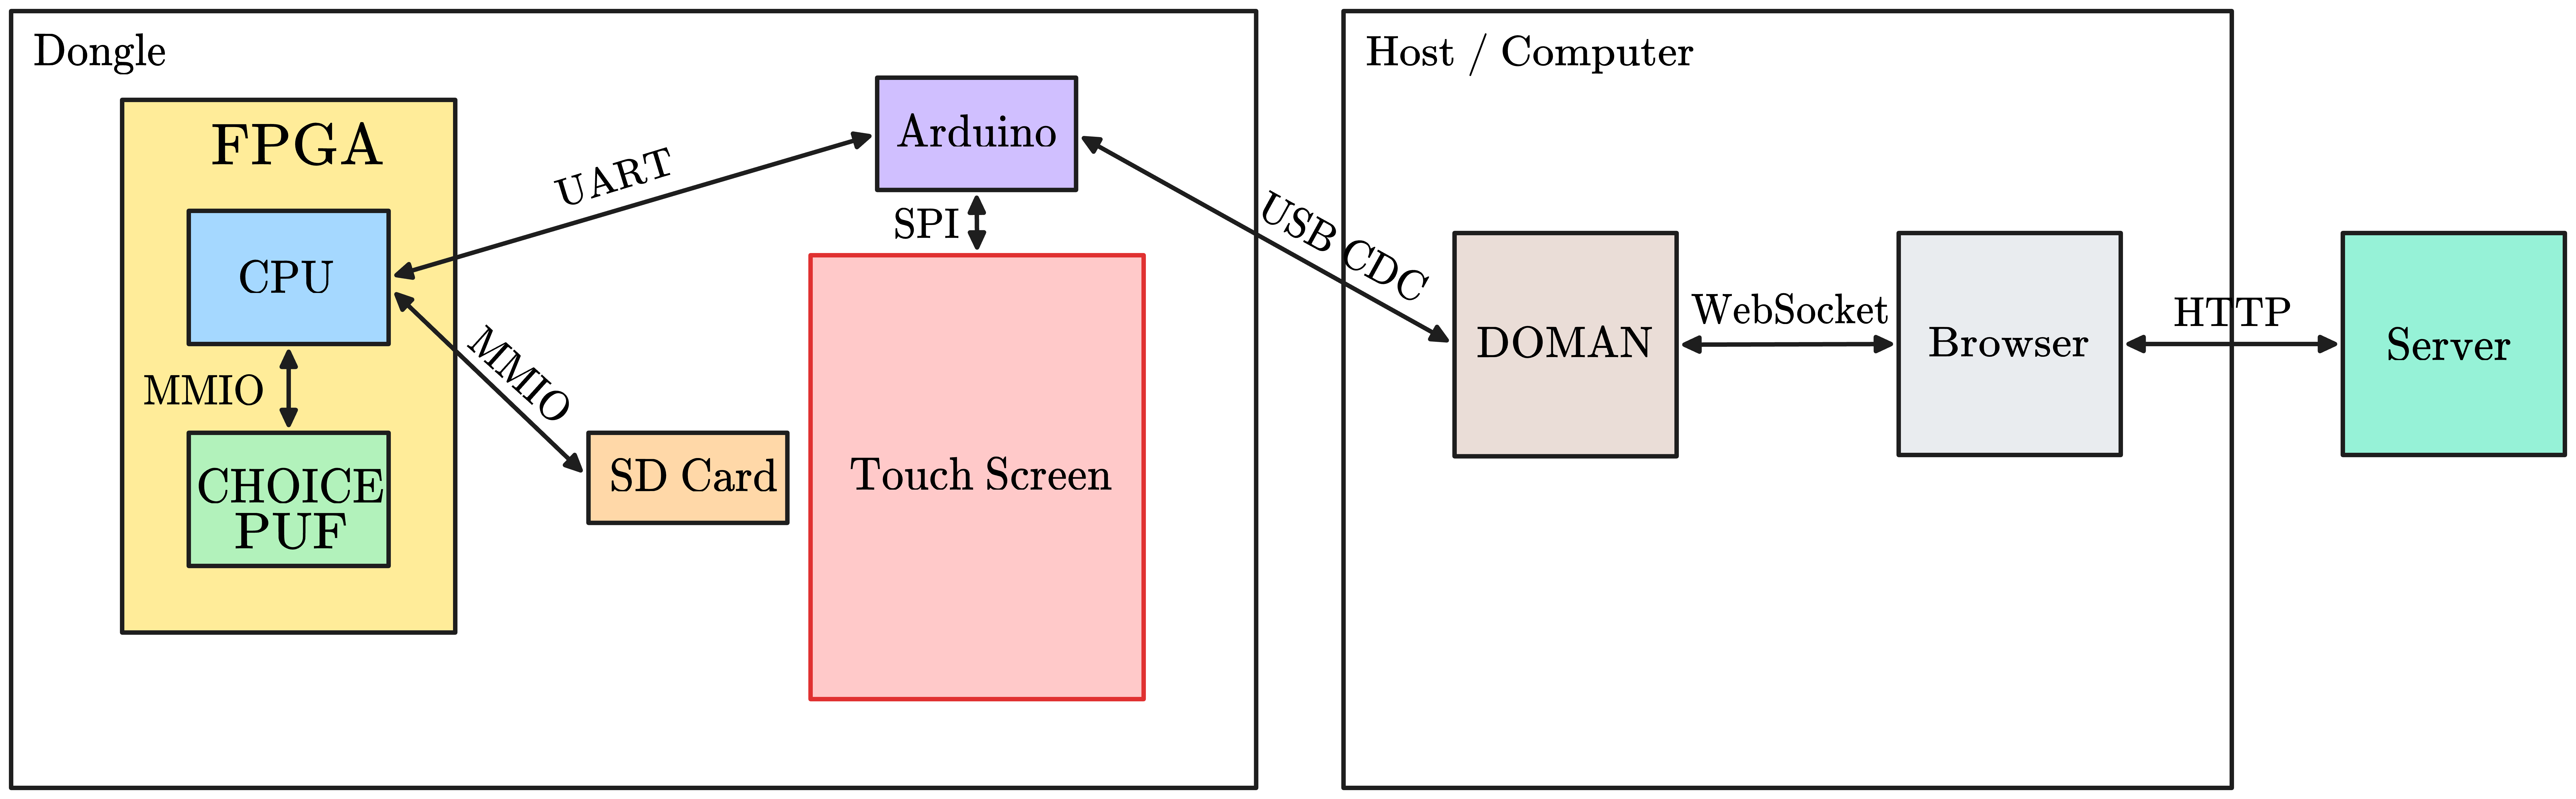
\includegraphics[width=\linewidth]{img/system-implementation.png}
    \caption{Physical implementation components}
    \label{fig:physical-implementation}
\end{figure}

The FPGA and the Arduino communicate over UART using a custom binary framing protocol that will be explained later. The FPGA implements the CPU and the CHOICE PUF, both of which are defined using Verilog and VHDL respectively. The CHOICE PUF and the SD card are exposed as peripherals to the CPU and communication is done via MMIO (Memory-Mapped I/O). The FPGA-defined CPU is used to augment the CHOICE PUF to an LR-PUF by carrying out the necessary hashing and storing of the states on the SD card. The Arduino board communicates with the touch screen via SPI (Serial Peripheral Interface). The Arduino communicates with the computer via DOMAN over a USB CDC (Universal Serial Bus Communications Device Class) serial port. DOMAN is a local server that exposes a WebSocket endpoint that the Javascript on the browser uses to talk to the dongle. The browser communicates with the server via HTTP since actually the server in this implementation is running locally on the host for test purposes.
\section{Dongle Implementation}
A picture of the actual dongle can be seen in figure \ref{fig:real-dongle}. The two buttons next to the touch screen are optional and could be used later for accepting or refusing the sensitive requests.

\begin{figure}
    \centering
    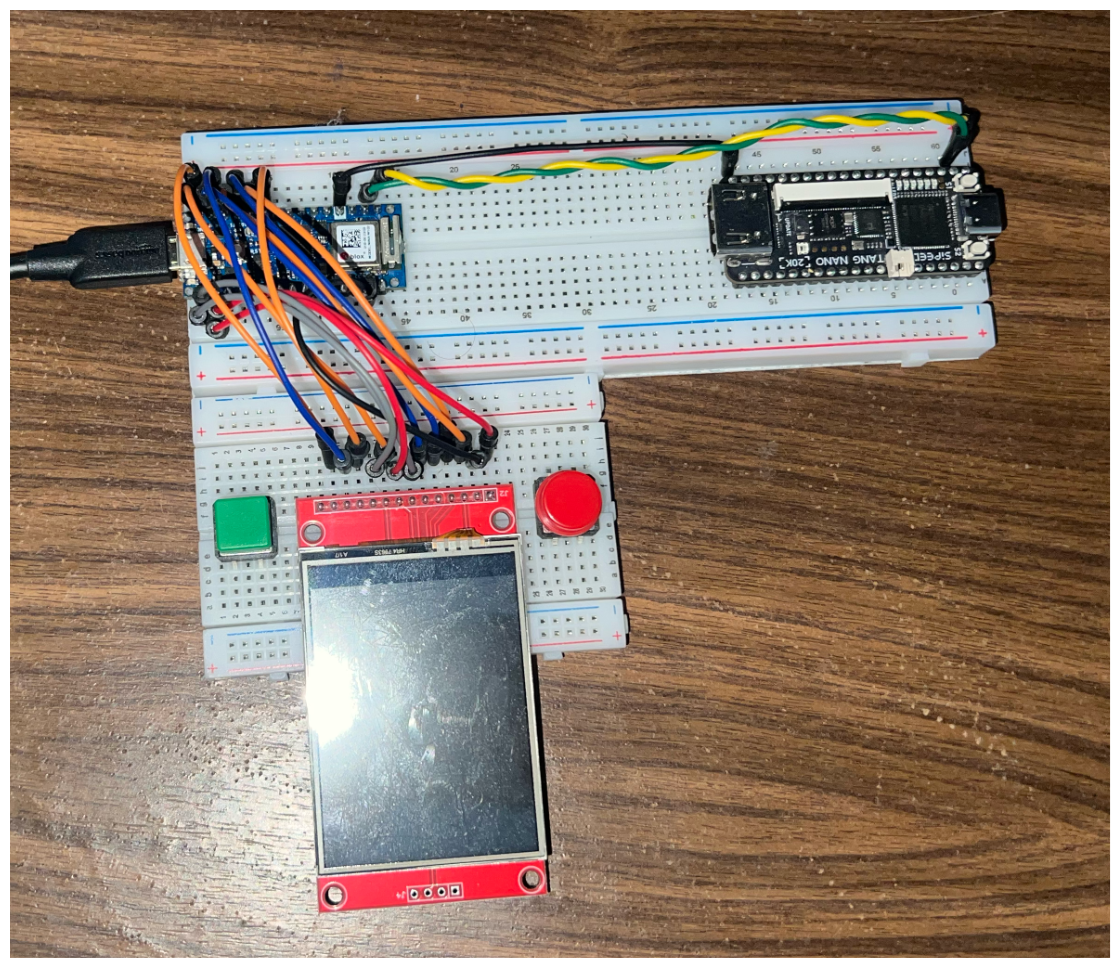
\includegraphics[width=0.6\linewidth]{img/real-dongle.png}
    \caption{Picture of the dongle}
    \label{fig:real-dongle}
\end{figure}

The FPGA part of the dongle handles the LR-PUF logic, whilst the Arduino handles communication with the host computer, cryptographic operations and drives the touch screen display. The raw CHOICE-PUF responses never exit the fabric of the FPGA, rather the Arduino has a list of commands it can issue to the FPGA to only carry out the necessary LR-PUF logic.


\subsection{FPGA Implementation}
The code for the FPGA implementation including the firmware can be found in the repository titled \verb|REPUSH-FPGA|, the \verb|README| file of the repository describes the project structure and how to compile, synthesize and flash the FPGA with the implementation.

The used FPGA board is a Sipeed Tang Nano 20k development board \cite{sipeed_tang_nano_20k} which hosts a Gowin GW2AR-18 FPGA chip. The implemented CPU is a PicoRV32 RISC-V core \cite{picoRV32} defined in Verilog. The CPU implementation and the firmware for it was originally taken from \cite{picorv32_tang_nano_unified} and expanded to accommodate the CHOICE-PUF as a peripheral and carry out all the necessary LR-PUF operations. The CHOICE-PUF VHDL implementation was taken from the Github repository \cite{choice_puf_repo} mentioned in the CHOICE-PUF paper \cite{9556423} and was modified to work on the targeted GW2AR-18 FPGA chip since the original implementation was meant for a Xilinx FPGA, a controller state-machine was added to control the CHOICE-PUF via MMIO from the CPU.

\subsubsection{PicoRV32 Core Configuration}
The PicoRV32 core is instantiated with the parameters listed in table \ref{tab:picorv32-params}. The CPU runs at a frequency of 9 MHz which is obtained from the 27 MHz oscillator of the board using the on-chip rPLL (rational Phase-Locked Loop). The CPU has access to 64 KB of SRAM defined using $\verb|SRAM_ADDR_WIDTH|=14$, which gives $2^{14}=65\,536~bytes$. Since the SRAM serves as both instruction memory and data memory within a fixed-size region, there is no heap and would-be dynamic allocations are replaced with static global variables. The compiled firmware occupies around 61 KB of the 64 KB SRAM. It is loaded at address \verb|PROGADDR_RESET = 0x00000000| and that is where the CPU begins executing the instructions at boot and on reset. Multiplication and division instructions were enabled since the firmware needs them for array indexing among other things. The stack starts at the top of the SRAM at address \verb|STACKADDR = 0x00010000| and grows downward, leaving only 3.2 KB of headroom for the stack. In practice, this small size proved to be sufficient. The barrel shifter and compressed ISA (Instruction Set Architecture) are disabled to reduce the footprint of the CPU on the FPGA. 

\begin{table}[ht!]
\centering
\caption{PicoRV32 parameters.}
\begin{tabular}{lll}
\hline
\textbf{Parameter} & \textbf{Value} & \textbf{Description} \\
\hline
Clock frequency     & 9~MHz          & Derived from 27~MHz crystal via rPLL \\
\texttt{SRAM\_ADDR\_WIDTH} & 14      & 64~KB combined instruction/data memory \\
\texttt{ENABLE\_MUL}       & 1       & Hardware 32$\times$32 multiplier \\
\texttt{ENABLE\_DIV}       & 1       & Hardware divider \\
\texttt{BARREL\_SHIFTER}   & 0       & Disabled; reduces LUT count \\
\texttt{COMPRESSED\_ISA}& 0       & 32-bit instructions (no RV32C compression) \\
\texttt{PROGADDR\_RESET}   & \texttt{0x00000000} & Boot vector (bottom of SRAM) \\
\texttt{STACKADDR}         & \texttt{0x00010000} & Initial stack pointer (top of SRAM) \\
\hline
\end{tabular}
\label{tab:picorv32-params}
\end{table}

\subsubsection{Memory-Mapped I/O}
As mentioned before, the CPU uses MMIO to interact with the CHOICE PUF and other peripherals. As seen in table \ref{tab:mmio-map}, each peripheral is assigned a fixed address range. When the CPU wants to use a peripheral, it puts its address on the bus \verb|mem_addr|, the data to write on \verb|mem_wdata|, and raises the \verb|mem_valid| signal. Once the \verb|mem_valid| signal is raised, every peripheral compares the value inside \verb|mem_addr| with its address range and the one whose range matches it raises its select signal. If it is a write transaction, the peripheral reads the data from \verb|mem_wdata| and acts on it. If it is a read transaction, the peripheral places its response on \verb|mem_rdata| for the CPU to read back. Once the peripheral has finished its task, it raises its ready signal which feeds into \verb|mem_ready|. The CPU stalls until \verb|mem_ready| goes high. 

\begin{table}[ht!]
\centering
\caption{MMIO address map.}
\begin{tabular}{lll}
\hline
\textbf{Address range} & \textbf{Peripheral} & \textbf{Description} \\
\hline
\texttt{0x00000000}--\texttt{0x0000FFFF} & SRAM            & 64~KB program and data memory \\
\texttt{0x80000000}                      & LEDs            & 6-bit on-board LED register \\
\texttt{0x80000008}--\texttt{0x8000000F} & Debug UART      & Serial console (TX/RX) \\
\texttt{0x80000010}                      & Countdown timer & Hardware timeout counter \\
\texttt{0x80000020}                      & WS2812b         & Addressable RGB LED driver \\
\texttt{0x80000030}--\texttt{0x8000003F} & SD SPI helper   & Byte-level SPI controller for SD card \\
\texttt{0x80000040}--\texttt{0x8000004F} & CHOICE-PUF      & PUF command/response registers \\
\texttt{0x80000058}--\texttt{0x8000005F} & Arduino UART    & UART to the Arduino board (TX/RX) \\
\hline
\end{tabular}
\label{tab:mmio-map}
\end{table}

The CHOICE PUF peripheral at base address \verb|0x80000040| exposes three 32-bit registers (Table \ref{tab:puf-regs}). Since the PicoRV32 is a 32-bit CPU and can only transfer 32 bits per transaction, the 64-bit command and response are each split across two buses that share the same addresses. Commands are written to \verb|payload_hi| and \verb|payload_lo|, where the top four bits of \verb|payload_hi| determine the command type (request measurement, set choice, set address tuning or load a pattern) and the parameters are passed in \verb|payload_lo|. Writing to the trigger register at \verb|0x80000048| executes the command defined within the buses. For reading the PUF's response, the firmware polls the status register at the same address \verb|0x80000048| until its bit[0] is set to 1 by the PUF to indicate that the 64-bit response of the PUF is accessible on \verb|0x80000040| and \verb|0x80000044| via the two buses \verb|response_hi| and \verb|response_lo|.


\begin{table}[ht!]
  \centering
  \caption{CHOICE-PUF peripheral address map.}
  \begin{tabular}{llll}
  \hline
  \textbf{Offset} & \textbf{Address} & \textbf{Write} & \textbf{Read} \\
  \hline
  \texttt{0x0} & \texttt{0x80000040} & \texttt{payload\_hi}: command bits [63:32]       & \texttt{response\_hi}: response [63:32] \\
  \texttt{0x4} & \texttt{0x80000044} & \texttt{payload\_lo}: command bits [31:0]         & \texttt{response\_lo}: response [31:0] \\
  \texttt{0x8} & \texttt{0x80000048} & \texttt{trigger}: a write executes the command    & \texttt{status}: bit[0]=1 if response ready \\
  \hline
  \end{tabular}
  \label{tab:puf-regs}
  \end{table}

\subsubsection{CHOICE-PUF Implementation}
The CHOICE-PUF VHDL implementation was taken from \cite{choice_puf_repo} and adapted to run on the GW2AR-18. In the original code, each PUF cell used 32-bit ASRs, which gave it a challenge space of $\binom{4}{2} \cdot 32^2 = 6144$ challenges. To reduce the footprint of the PUF on the FPGA, the ASRs were reduced to 8 bits, which reduced the challenge space to $\binom{4}{2} \cdot 8^2 = 384$ challenges. The PUF response width was also reduced from 128 bits to 64 bits to make it fit in the GW2AR-18.

The original CHOICE-PUF VHDL implementation was designed for a Xilinx Spartan-3E FPGA and relied on Xilinx-specific features that needed to be replaced with their Gowin counterparts:
\begin{itemize}
    \item \textbf{Shift register LUT primitives (\texttt{SRLC32E})}: The original ASRs were implemented using Xilinx \texttt{SRLC32E} primitives. Since no equivalent primitive exists on the GW2AR-18, they were replaced with 8-bit ASRs described behaviorally in VHDL.
    \item \textbf{Carry chain primitives (\texttt{CARRY4})}: The original implementation used the Xilinx \texttt{CARRY4} primitive to chain the four ASR outputs through a carry chain. On the GW2AR-18, this was replaced with four of Gowin's native \texttt{ALU} components configured as full adders and chained together by connecting the \verb|COUT| of each instance to the \verb|CIN| of the next.
    \item \textbf{Output flip-flop (\texttt{FDPE})}: The Xilinx \texttt{FDPE} primitive is a D flip-flop with an asynchronous preset input that captures the outcome of the carry chain race, i.e. the output of the PUF cell. It was replaced with a behavioral description thereof. 
    \item \textbf{Synthesis attributes}: Xilinx's \texttt{DONT\_TOUCH} attribute prevented the synthesizer from simplifying or removing the carry chain structure within each PUF cell. The attribute was replaced with Gowin's attribute \texttt{syn\_dont\_touch} to prevent signals from being optimized or merged. \texttt{syn\_preserve} is used to keep the \texttt{ALU} instances intact. To avoid merging the PUF cells, \texttt{KEEP\_HIERARCHY} is applied to all PUF cell instances.
\end{itemize}

A Verilog module \texttt{puf\_peripheral.v} was written to wrap the CHOICE PUF and expose it as an MMIO peripheral to the CPU. It implements a finite state-machine that sends commands to the PUF controller and writes the PUF response back on the response registers for the CPU to read.




\subsubsection{Firmware}
The FPGA CPU's firmware is written in C and the CHOICE-PUF is exposed as a memory-mapped peripheral at a fixed base address. The firmware configures it by writing tuning and choice registers, then reads the 64-bit response by issuing a measurement request and polling a ready flag. For hashing operations, the firmware uses the BLAKE2b \cite{rfc7693} hashing function from the Monocypher library \cite{monocypher}. The states of the LR-PUF and the CA's public key are stored in an SD card inserted into the FPGA board's SD card slot, which is also exposed to the CPU via MMIO. 

For BCH error correction, the implementation was ported from the Linux kernel implementation \texttt{lib/bch.c} \cite{linux_bch}. BCH codes are parameterized by  $m$ and $T$, where $m$ is the order of the Galois field $GF(2^m)$. The Galois field allows for polynomial arithmetic which has the properties that make error correction possible. The maximum codeword's length is given by $2^m-1$, and $T$ is the maximum number of bit flips the code can correct. The parameters $m=7$ and $T=4$ were chosen, giving a $BCH(cd_{len}=127, m_{len}=99, T=4)$ where:
\begin{itemize}
    \item The maximum codeword length is $cd_{len}= 2^m-1= 2^7 -1 = 127~bits$.
    \item The maximum message length is $m_{len}=127 - m\cdot T = 127 - 7\cdot4 = 99~bits$.
    \item The parity bits length is $ECC_{len}=m\cdot T = 7\cdot4=28 ~bits$. 
\end{itemize}
Since the CHOICE PUF returns a response of 64 bits, only 64 bits of the message length $m_{len} = 99~bits$ are used and the remaining 35 leading bits are set to 0. The correction capability of $T=4$ is sufficient given the stability of the CHOICE PUF under majority voting. The vote count for majority voting was chosen as 10. Since the FPGA CPU has no heap access, all dynamic memory allocations from the Linux BCH implementation were replaced with static global variables. 
To encode the data and get the parity bits $ECC$, the polynomial remainder operation $ECC(x) = D(x) \cdot x^{28} \mod g(x)$ must be performed, where $D(x)$ is the data polynomial and $g(x)$ is the generator polynomial. There are multiple ways to compute this remainder efficiently. The original Linux kernel implementation used a table-based encoder which processes the data 8 bits at a time using precomputed lookup tables. This approach is fast but it requires storing the table in RAM via dynamic memory allocation, which is unavailable here since there is no heap. Instead, the BCH encoding function was adapted to use a bit-by-bit LFSR (Linear Feedback Shift Register) encoder which processes the data one bit at a time to compute the remainder $ECC(x)$. While this new approach is slower, it does not require RAM, and it is still sufficiently fast given the small 64-bit data size that has to be encoded.

\subsubsection{Resource Utilization}
Table \ref{tab:fpga-resources} shows the resource utilization of the FPGA implementation. 

\begin{table}[ht!]
\centering
\caption{FPGA resource utilization}
\begin{tabular}{llll}
\hline
\textbf{Resource} & \textbf{Used} & \textbf{Available} & \textbf{Utilization} \\
\hline
Logic cells (total)  & 12\,223 & 20\,736 & 59\% \\
\quad -- LUT         & 10\,944 & ---     & ---  \\
\quad -- ALU         &  1\,135 & ---     & ---  \\
\quad -- SSRAM       &     24  & ---     & ---  \\
Flip-flops (Logic FF)&  3\,863 & 15\,552 & 25\% \\
CLS                  &  6\,859 & 10\,368 & 67\% \\
BSRAM (SDPB)         &     33  &     46  & 72\% \\
I/O Ports            &     18  &     66  & 28\% \\
\hline
\end{tabular}
\label{tab:fpga-resources}
\end{table}

\subsection{Communication protocol}

\begin{figure}
    \centering
    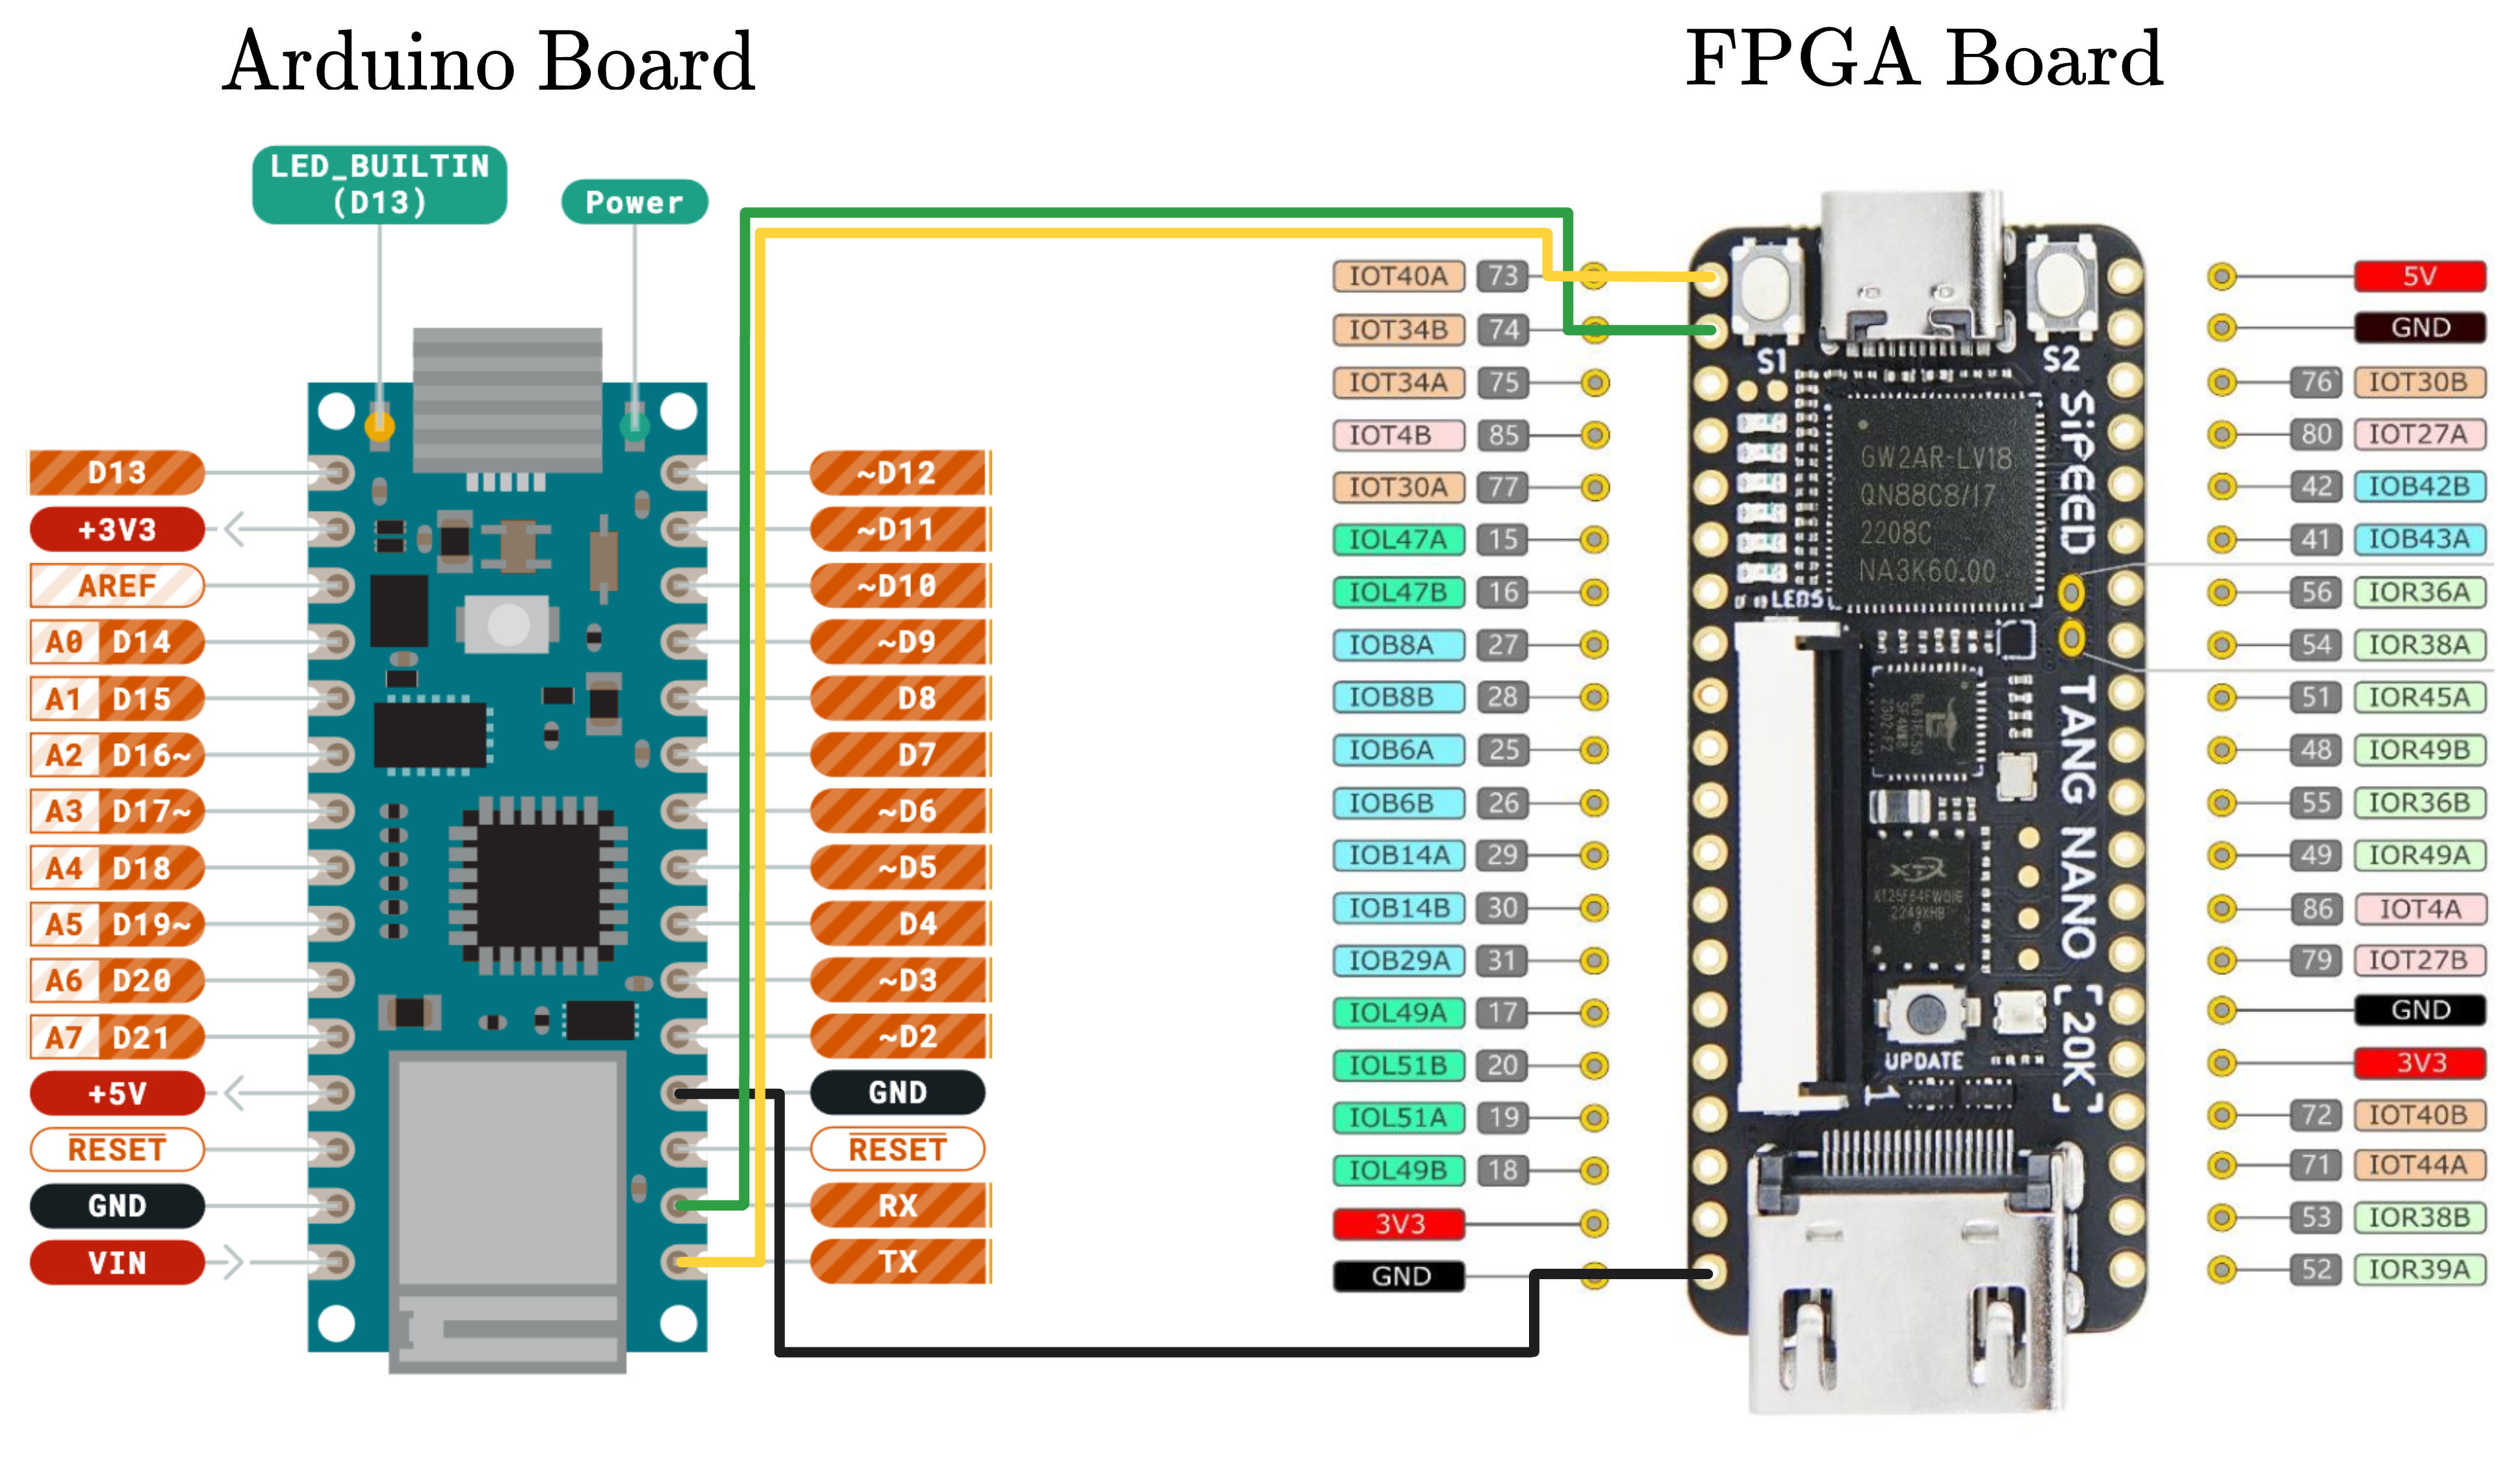
\includegraphics[width=1\linewidth]{img/arduino2fpga.png}
    \caption{UART connection between the Arduino board and the FPGA board}
    \label{fig:uart-arduino-fpga}
\end{figure}

The Arduino must communicate with the FPGA in order to manage the states and the LR-PUF and to carry out the necessary logic of the protocol. The FPGA and the Arduino exchange messages using a custom framing protocol layered on top of the UART.
Each frame has the structure shown in Table \ref{tab:proto-frame}.  There are two fields dedicated to the start-of-frame SOF1 and SOF2. This is done so as to reduce the probability of noise being taken as the start of a frame. Using only one field, that probability would be $1/256$, but with two fields it becomes $1/65536$ which is less likely. It also gives the parser the opportunity to re-synchronize after a corrupted or partial frame. A single SOF byte would not be reliable for this since it could randomly appear in corrupted data, but two consecutive bytes matching both SOF1 and SOF2 are less likely to appear.

The default Arduino RX and TX pins are connected to pins 74 and 73 of the FPGA board respectively, as seen in Figure \ref{fig:uart-arduino-fpga}.

\begin{table}[ht!]
\centering
\caption{FPGA protocol frame layout.}
\begin{tabular}{lll}
\hline
\textbf{Field} & \textbf{Size (bytes)} & \textbf{Description} \\
\hline
SOF1            & 1 & Start-of-frame marker (0xA5) \\
SOF2            & 1 & Start-of-frame marker (0x5A) \\
Version         & 1 & Protocol version (currently 1) \\
Message type    & 1 & REQ (1), RSP (2), or ERR (3) \\
Sequence number & 1 & Monotonically incrementing per call \\
Command         & 1 & Command identifier (Table~\ref{tab:proto-cmds}) \\
Payload length  & 2 & Little-endian, maximum 96 bytes \\
Payload         & 0--96 & Command-specific data \\
CRC16           & 2 & CRC-16/IBM over all fields after SOF \\
\hline
\end{tabular}
\label{tab:proto-frame}
\end{table}


The command identifiers used by the REPUSH-specific LR-PUF subsystem are listed in Table~\ref{tab:proto-cmds}. This is what the Arduino can tell the FPGA to do.

  \begin{table}[ht!]
  \centering
  \caption{LR-PUF commands descriptions}
  \begin{tabular}{cll}
  \hline
  \textbf{ID} & \textbf{Command} & \textbf{Purpose} \\
  \hline
  4  & \texttt{GET\_CA\_KEY}             & Retrieve the CA public key stored on the FPGA \\
  5  & \texttt{PUF\_GET\_FREE\_STATE}    & Return the index of an unoccupied state slot \\
  6  & \texttt{PUF\_RECONFIGURE\_STATE}  & Derive a new domain state $S^{Domain}_{i+1}$ \\
  8  & \texttt{PUF\_SET\_DOMAIN}         & Associate a domain string with a state slot \\
  9  & \texttt{PUF\_STORE\_ENROLLMENT}   & Write pubkey, challenge, and server key to a slot \\
  10 & \texttt{PUF\_SAVE\_STATES}        & Flush all state slots from RAM to SD card \\
  11 & \texttt{PUF\_FIND\_STATE\_BY\_DOMAIN} & Look up a slot by domain string \\
  12 & \texttt{PUF\_MARK\_ACKNOWLEDGED}  & Set the acknowledged flag for a slot / state \\
  13 & \texttt{PUF\_CLEAR\_STATES}       & Erase all state slots (debug use) \\
  14 & \texttt{PUF\_GET\_SLOT\_STATUS}   & Query the status and domain of a single slot / state \\
  15 & \texttt{PUF\_BCH\_ENROLL}         & Majority-vote PUF measurement and compute BCH helper data \\
  16 & \texttt{PUF\_BCH\_QUERY}          & Re-derive PUF response using BCH error correction \\
  \hline
  \end{tabular}
  \label{tab:proto-cmds}
  \end{table}

The structure of the payloads and responses of the commands can be found in table \ref{tab:proto-cmds-struct}. Some unused utility commands for debug purposes are also implemented and are found in table \ref{tab:proto-util-cmds}.

  \begin{table}[ht!]
  \centering
  \caption{LR-PUF commands payload and response structures (B stands for bytes)}
  \begin{tabular}{clll}
  \hline
  \textbf{ID} & \textbf{Command} & \textbf{Payload} & \textbf{Response} \\
  \hline
  4  & \texttt{GET\_CA\_KEY} & Empty & 32B pubkey \\
  5  & \texttt{PUF\_GET\_FREE\_STATE} & Empty & 1B state index \\
  6  & \texttt{PUF\_RECONFIGURE\_STATE} & State (1B) + seed (4B) & Empty \\
  8  & \texttt{PUF\_SET\_DOMAIN} & State (1B) + domain (var, max 63B) & Empty \\
  9  & \texttt{PUF\_STORE\_ENROLLMENT} & State + keys (81B total) & Empty \\
  10 & \texttt{PUF\_SAVE\_STATES} & Empty & Empty \\
  11 & \texttt{PUF\_FIND\_STATE\_BY\_DOMAIN} & Domain (var, max 63B) & 81B state data \\
  12 & \texttt{PUF\_MARK\_ACKNOWLEDGED} & State (1B) & Empty \\
  13 & \texttt{PUF\_CLEAR\_STATES} & Empty & Empty \\
  14 & \texttt{PUF\_GET\_SLOT\_STATUS} & State (1B) & Status (2B) + domain (max 63B) \\
  15 & \texttt{PUF\_BCH\_ENROLL} & State (1B) + ID (4B) + count (1B) & 32B enrolled key \\
  16 & \texttt{PUF\_BCH\_QUERY} & State (1B) + ID (4B) & 32B corrected key \\
  \hline
  \end{tabular}
  \label{tab:proto-cmds-struct}
  \end{table}


\begin{table}[ht!]
\centering
\caption{Utility commands}
\begin{tabular}{clll}
\hline
\textbf{ID} & \textbf{Command} & \textbf{Request} & \textbf{Response} \\
\hline
1 & \texttt{PING} & 4B string ``PING'' & Echo ``PING'' \\
2 & \texttt{GET\_INFO} & Empty & 8B+ (version, max payload, features) \\
3 & \texttt{GET\_TIME} & Empty & 4B timestamp \\
\hline
\end{tabular}
\label{tab:proto-util-cmds}
\end{table}

The Arduino initiates every exchange with a REQ frame and waits for a matching RSP or ERR frame identified by the same sequence number and command. 

An example request from the Arduino to the FPGA follows this sequence:
\begin{enumerate}
      \item The Arduino constructs a REQ frame which contains the command ID,
      a monotonically incrementing sequence number, and the command-specific payload.

      \item The Arduino flushes the UART RX buffer, sends the REQ frame, and enters a
      receive loop with a per-command timeout which ranges from one second for simple queries to 17 seconds for BCH enrollment with majority voting.

      \item The FPGA parses the incoming frame, validates the CRC, and executes the command.

      \item FPGA sends a response frame: either RSP on success or ERR on failure. The response carries the same sequence number
      and command ID as the request.

      \item Arduino's receive loop matches the response by checking
      \texttt{response.seq == request.seq} and \texttt{response.cmd == request.cmd}.
      Frames that do not match (e.g: stale output from a prior command) are discarded and
      the loop continues waiting. If the timeout expires without a matching frame, the
      Arduino retries with a fresh frame and a new sequence number, waiting
      150~ms before each retry. A maximum of 3 attempts are made in total, after which the call returns failure.
  \end{enumerate}

\subsection{Arduino Implementation}
The Arduino implementation is written in C++ and the PlatformIO IDE solution \cite{platformio_ide} was used for managing the project. The used Arduino board is an Arduino Nano 33 IoT \cite{arduino_nano_33_iot}.

\subsubsection{Commands}
The Arduino exposes the high-level commands in table \ref{tab:arduino-commands} via its USB serial interface, which DOMAN uses.

\begin{table}[ht!]
\centering
\caption{High-level commands from DOMAN to Arduino}
\begin{tabular}{lll}
\hline
\textbf{Command} & \textbf{Arguments} & \textbf{Purpose} \\
\hline
\texttt{enroll} & Certificate, Payload & Phase 1: Perform enrollment (Algorithm \ref{alg:dongle-enroll}) \\
\texttt{sign\_payload} & Domain, Payload & Phase 2: Sign non-sensitive request \\
\texttt{sign\_sensitive} & Domain, Payload & Phase 2: Sign sensitive request with user approval \\
\texttt{reconf} & Domain, Payload & Phase 3: Rotate key and reconfigure state \\
\texttt{acknowledge} & Domain, Signature & Phase 1: Acknowledge server-signed enrollment \\
\texttt{reconf\_ack} & Domain, Signature & Phase 3: Acknowledge server-signed reconfiguration \\
\texttt{ready} & — & Poll dongle availability (returns ``READY'') \\
\hline
\end{tabular}
\label{tab:arduino-commands}
\end{table}



In addition to the main protocol commands, the Arduino implements several debug commands for testing and development. The most commonly used state management debug commands are in table \ref{tab:debug-commands}.

\begin{table}[ht!]
\centering
\caption{State management debug commands}
\begin{tabular}{lll}
\hline
\textbf{Command} & \textbf{Arguments} & \textbf{Purpose} \\
\hline
\texttt{fp\_list\_states} & — & List all 11 state slots with their domain, \\
&  & initialization status, and acknowledgment flag \\
\texttt{fp\_clear\_states} & — & Erase all state slots from FPGA memory \\
&  & (resets dongle to factory state) \\
\hline
\end{tabular}
\label{tab:debug-commands}
\end{table}

\subsubsection{Cryptographic Schemes}
The Arduino implementation employs four cryptographic primitives:

\textbf{1. Ed25519: Edwards-Curve Digital Signature Algorithm}: A cryptographic signature scheme defined in RFC 8032 \cite{rfc8032}. The dongle uses the Ed25519 functions from the Arduino Cryptography Library \cite{arduinolibs_crypto}:
\begin{itemize}
    \item \texttt{Ed25519::sign(signature, privateKey, publicKey, message, messageLen)}: Signs a message with the private key.
    \item \texttt{Ed25519::verify(signature, publicKey, message, messageLen)}: Verifies a signature against a public key.
    \item \texttt{Ed25519::derivePublicKey(publicKey, privateKey)}: Derives the public key from a private key.
\end{itemize}
It is used during phase 1 to verify $[LoginPayload]_{SK_{\text{Server}}}$, to sign $[LoginPayload]_{SK_0}$ and verify the server's acknowledgment $LoginAck$. During phase 2, it is used to sign sensitive and non-sensitive requests $[SignaturePayload]_{SK_i}$ and $[SensitivePayload]_{SK_i}$. And during phase 3, to sign the reconfiguration token  ($[PK_{i+1} \| ReconfPayload]_{SK_i}$) and verify the server's acknowledgment $ReconfAck$.

\textbf{2. Curve25519 (X25519): Elliptic Curve Diffie-Hellman}: an elliptic curve designed for ECDH key agreement, defined in RFC 7748 \cite{rfc7748}. The following functions from the Arduino Cryptography Library are used:
\begin{itemize}
    \item \texttt{Curve25519::dh1(publicKey, privateKey)}: Generates the public key from a private key.
    \item \texttt{Curve25519::dh2(sharedSecret, privateKey)}: Computes the shared secret via scalar multiplication.
\end{itemize}
The exact usage for ECDH is explained in the next section below.

\textbf{3. ChaCha20-Poly1305: Authenticated Encryption with Associated Data (AEAD)}: A combined encryption and authentication scheme defined in RFC 7539 \cite{rfc7539}. It combines ChaCha20, which is a stream cipher, and Poly1305, which is a one-time authenticator. ChaCha20 handles confidentiality by encrypting the plain text and Poly1305 handles integrity by detecting if the cipher text was tampered with in-transit. The following functions from the Arduino Cryptography Library are used:
\begin{itemize}
    \item \texttt{ChaChaPoly::setKey(key, keyLen)}: Sets the 32-byte encryption key.
    \item \texttt{ChaChaPoly::setIV(iv, ivLen)}: Sets the 12-byte nonce.
    \item \texttt{ChaChaPoly::encrypt(ciphertext, plaintext, plaintextLen)}: Encrypts the plaintext.
    \item \texttt{ChaChaPoly::computeTag(tag, tagLen)}: Computes the 16-byte Poly1305 tag.
\end{itemize}
ChaCha20-Poly1305 is used during phase 1 to encrypt the $LoginToken$ and in phase 3 to encrypt the $ReconfToken$.

\textbf{4. SHA-256: Secure Hash Algorithm}: A cryptographic hash function defined in the FIPS 180-4 standard \cite{fips180_4}. The following functions from the Arduino Cryptography Library are used:
\begin{itemize}
    \item \texttt{SHA256::reset()}: Initializes the hash state.
    \item \texttt{SHA256::update(data, dataLen)}: Feeds data into the hash function (can be called multiple times for streaming).
    \item \texttt{SHA256::finalize(digest, digestLen)}: Completes the hash and returns the 32-byte digest.
\end{itemize}
SHA-256 is used for deriving the symmetric encryption key from the ECDH shared secret during phase 1 and phase 3 as explained in the next section below.




\subsubsection{Usage of ECIES (Elliptic Curve Integrated Encryption Scheme) for Encryption}
There is a slight deviation from the protocol design when it comes to encryption since the Ed25519 public key provided by the server $PK_{\text{Server}}^{\text{Ed25519}}$ can only be used for verifying signatures and not for encryption. Using ECIES we can use the provided server public key to encrypt a message that only the server could decrypt. ECIES is used during phase 1 to encrypt the $LoginToken$ and during phase 3 to encrypt the $ReconfToken$.

To explain how ECIES works in the technical implementation, the following notations are used:
\begin{itemize}
    \item $\text{Ed25519\_to\_X25519}(PK^{\text{Ed25519}})$: Function to convert an Ed25519 public key to X25519.
    \item $\text{X25519}(sk, pk)$: X25519 scalar multiplication to compute the shared secret from private key $sk$ and public key $pk$.
    \item $\text{SHA256}(m)$: SHA256 hash function.
    \item $\text{ChaCha20-Poly1305.Encrypt}(key, nonce, plaintext)$: ChaCha20 encryption with Poly1305 authentication.
    \item $\text{ChaCha20-Poly1305.Decrypt}(key, nonce, ciphertext, tag)$: ChaCha20 decryption with Poly1305 verification.
\end{itemize}

During phase 1, when the dongle needs to encrypt the $LoginToken$ which contains the username, password and $PK_0$ during $DongleEnroll$ (Algorithm \ref{alg:dongle-enroll}), it will follow the process described in the $ECIESEncrypt$ function defined in algorithm \ref{alg:ecies-encrypt-enroll}. It first takes the server's Ed25519 public key and converts it to an X25519 key suitable for ECDH (Elliptic Curve Diffie-Hellman), then it generates an ephemeral key pair, where the ephemeral public key is $eph\_pub=\text{X25519}(eph\_priv,G)$, with $G$ as the curve's base point. It then computes the ECDH shared secret as $shared\_secret=\text{X25519}(eph\_priv, PK_{\text{Server}}^{\text{X25519}})$, which is equivalent to $[a \cdot b]G$ where $a=eph\_priv$ and $b$ is the server's private scalar corresponding to its X25519 private key. The server will later be able to generate the shared secret using $shared\_secret=X25519(SK_{\text{Server}}, eph\_pub)$ due to the commutativity of elliptic curve scalar multiplication, in other words we would have:
$$
shared\_secret=\text{X25519}(a, [b]G) = \text{X25519}(b, [a]G) = [a \cdot b]G
$$
Where $a$ is the private scalar of the dongle and $b$ is the private scalar of the server.
Then a symmetric encryption key is derived by hashing the shared secret together with the ephemeral public key as $enc\_key=\text{SHA256}(shared\_secret||eph\_pub)$. Afterward, the plain text, which consists of the hex-encoded username, password and generated public key $PK_0$ separated by pipe characters, is encrypted using ChaCha20-Poly1305 with a randomly generated nonce, producing both a ciphertext and an authentication tag. Finally all sensitive intermediate values are deleted.

\begin{algorithm}[ht!]
\caption{$ECIESEncrypt(PK_{\text{Server}}^{\text{Ed25519}}, Username, Password, PK_0)$}
\begin{algorithmic}[1]
    \Require Server's Ed25519 public key $PK_{\text{Server}}^{\text{Ed25519}}$, user credentials $Username$ and $Password$, device generated public key $PK_{\text{0}}$.
    \Ensure  $(eph\_pub, nonce, ciphertext, tag)$ representing the encrypted LoginToken.

    \State $PK_{\text{Server}}^{\text{X25519}} \leftarrow \text{Ed25519\_to\_X25519}(PK_{\text{Server}}^{\text{Ed25519}})$

    \State $eph\_priv \leftarrow \text{TRNG}()$ \Comment{random 32-byte private key}
    \State $eph\_pub \leftarrow X25519(eph\_priv, \text{BasePoint})$ \Comment{derive public key}

    \State $shared\_secret \leftarrow \text{X25519}(eph\_priv, PK_{\text{Server}}^{\text{X25519}})$

    \State $enc\_key \leftarrow \text{SHA256}(shared\_secret \mathbin\| eph\_pub)$

    \State $plaintext \leftarrow \text{HexEncode}(Username) \,\|\, \texttt{"|"} \,\|\, \text{HexEncode}(Password) \,\|\, \texttt{"|"} \,\|\, \text{HexEncode}(PK_0)$

    \State $nonce \leftarrow \text{TRNG}()$ \Comment{12-byte IETF nonce}

    \State $(ciphertext, tag) \leftarrow \text{ChaCha20-Poly1305.Encrypt}(enc\_key, nonce, plaintext)$

    \State $\text{Wipe}(eph\_priv)$
    \State $\text{Wipe}(shared\_secret)$
    \State $\text{Wipe}(enc\_key)$
    \State $\text{Wipe}(plaintext)$

    \State \textbf{return} $(eph\_pub, nonce, ciphertext, tag)$
\end{algorithmic}
\label{alg:ecies-encrypt-enroll}
\end{algorithm}

The actual $LoginToken$ which will be transmitted to the server will have the following structure:
$$
LoginToken = eph\_pub \,\|\, nonce \,\|\, ciphertext \,\|\, tag
$$

The server decrypts the $LoginToken$ once it receives it during $VerifyLogin$ (Algorithm \ref{alg:verify-login}) by following the process outlined in $ECIESDecrypt$ (Algorithm \ref{alg:ecies-decrypt-enroll}). It begins by converting the server's Ed25519 private key to its X25519 equivalent and then reproduces the shared secret as $shared\_secret=\text{X25519}(SK_{\text{Server}}^{\text{X25519}},eph\_pub)$, which is equivalent to $[b \cdot a]G$ that is identical to the $[a \cdot b]G$ computed by the dongle as explained before. The symmetric key is then derived similarly as $enc\_key=\text{SHA256}(shared\_secret||eph\_pub)$. Decryption is then attempted using ChaCha20-Poly1305 and the authentication tag $auth\_valid$ is verified. If the tag check fails, the function fails to indicate that the token was tampered with in-transit. If the tag check is successful, the decrypted plain text is decoded to recover the username, password and $PK_0$. 

\begin{algorithm}[ht!]
\caption{$ECIESDecrypt(SK_{\text{Server}}^{\text{Ed25519}}, eph\_pub, nonce, ciphertext, tag)$}
\begin{algorithmic}[1]
    \Require Server's Ed25519 private key $SK_{\text{Server}}^{\text{Ed25519}}$, ephemeral public key $eph\_pub$, nonce, ciphertext, and authentication tag.
    \Ensure  Decrypted plaintext $(Username, Password, PK_0)$, or failure.
    \State $SK_{\text{Server}}^{\text{X25519}} \leftarrow \text{Ed25519\_to\_X25519}(SK_{\text{Server}}^{\text{Ed25519}})$
    \State $shared\_secret \leftarrow X25519(SK_{\text{Server}}^{\text{X25519}}, eph\_pub)$
    \State $enc\_key \leftarrow \text{SHA256}(shared\_secret \mathbin\| eph\_pub)$
    \State $(plaintext, auth\_valid) \leftarrow \text{ChaCha20-Poly1305.Decrypt}(enc\_key, nonce, ciphertext, tag)$
    \If{$auth\_valid = \textit{false}$}
        \State \textbf{return} ``Decryption failed: authentication tag verification failed''
    \EndIf
    \State $(Username, Password, PK_0) \leftarrow \text{HexDecode}(plaintext)$
    \State $\text{Wipe}(shared\_secret)$
    \State $\text{Wipe}(enc\_key)$
    \State \textbf{return} $(Username, Password, PK_0)$
\end{algorithmic}
\label{alg:ecies-decrypt-enroll}
\end{algorithm}

The same process for encrypting and decrypting is also used during phase 3 for encrypting and decrypting $ReconfToken$.

\subsubsection{Random Number Generation}
The Arduino must generate random numbers for three use-cases: the ephemeral keys for ECIES, nonces for ChaCha20-Poly1305 and for seeding the LR-PUF initial state $S_0$. Rather than relying on the Arduino's default weak \texttt{random()} function, another method was used.

The method was taken from \cite{rheingoldheavy2017better} and can be seen in the source code as the function \texttt{generateRandomSeed()}. It extracts randomness from an unconnected pin, in this case \texttt{A0} with the following steps:
\begin{enumerate}
    \item Read the analog pin 8 times and extract the least significant bit (LSB) of each reading
    \item Sum the 8 LSBs and take the parity (odd/even) as one random bit
    \item Assemble 8 parity bits into one byte
    \item Repeat 4 times to produce a 32-bit seed
\end{enumerate}

The entropy from thermal and electromagnetic noise on the unconnected analog pin is further amplified using this method. It is similar to how flipping a coin 8 times gives sequences that are less likely to be guessed.

\subsection{Touch Screen Implementation}
The dongle features a 2.4 inch TFT touch screen display with an ILI9341 display controller (Figure \ref{fig:tft-picture}). It has 240x320 pixels resolution in portrait orientation. The Arduino communicates with the display via SPI (Serial Peripheral Interface). As seen in table \ref{table:touchscreen-pins}, the SPI bus is shared between the display controller (ILI9341) and the touch controller (XPT2046) but the Arduino can choose which controller to address by pulling its CS (Chip select) line low. The touch screen implementation is initially based on the code from \cite{bytesnbits_spi_lcd_touchscreen}.

\begin{figure}
    \centering
    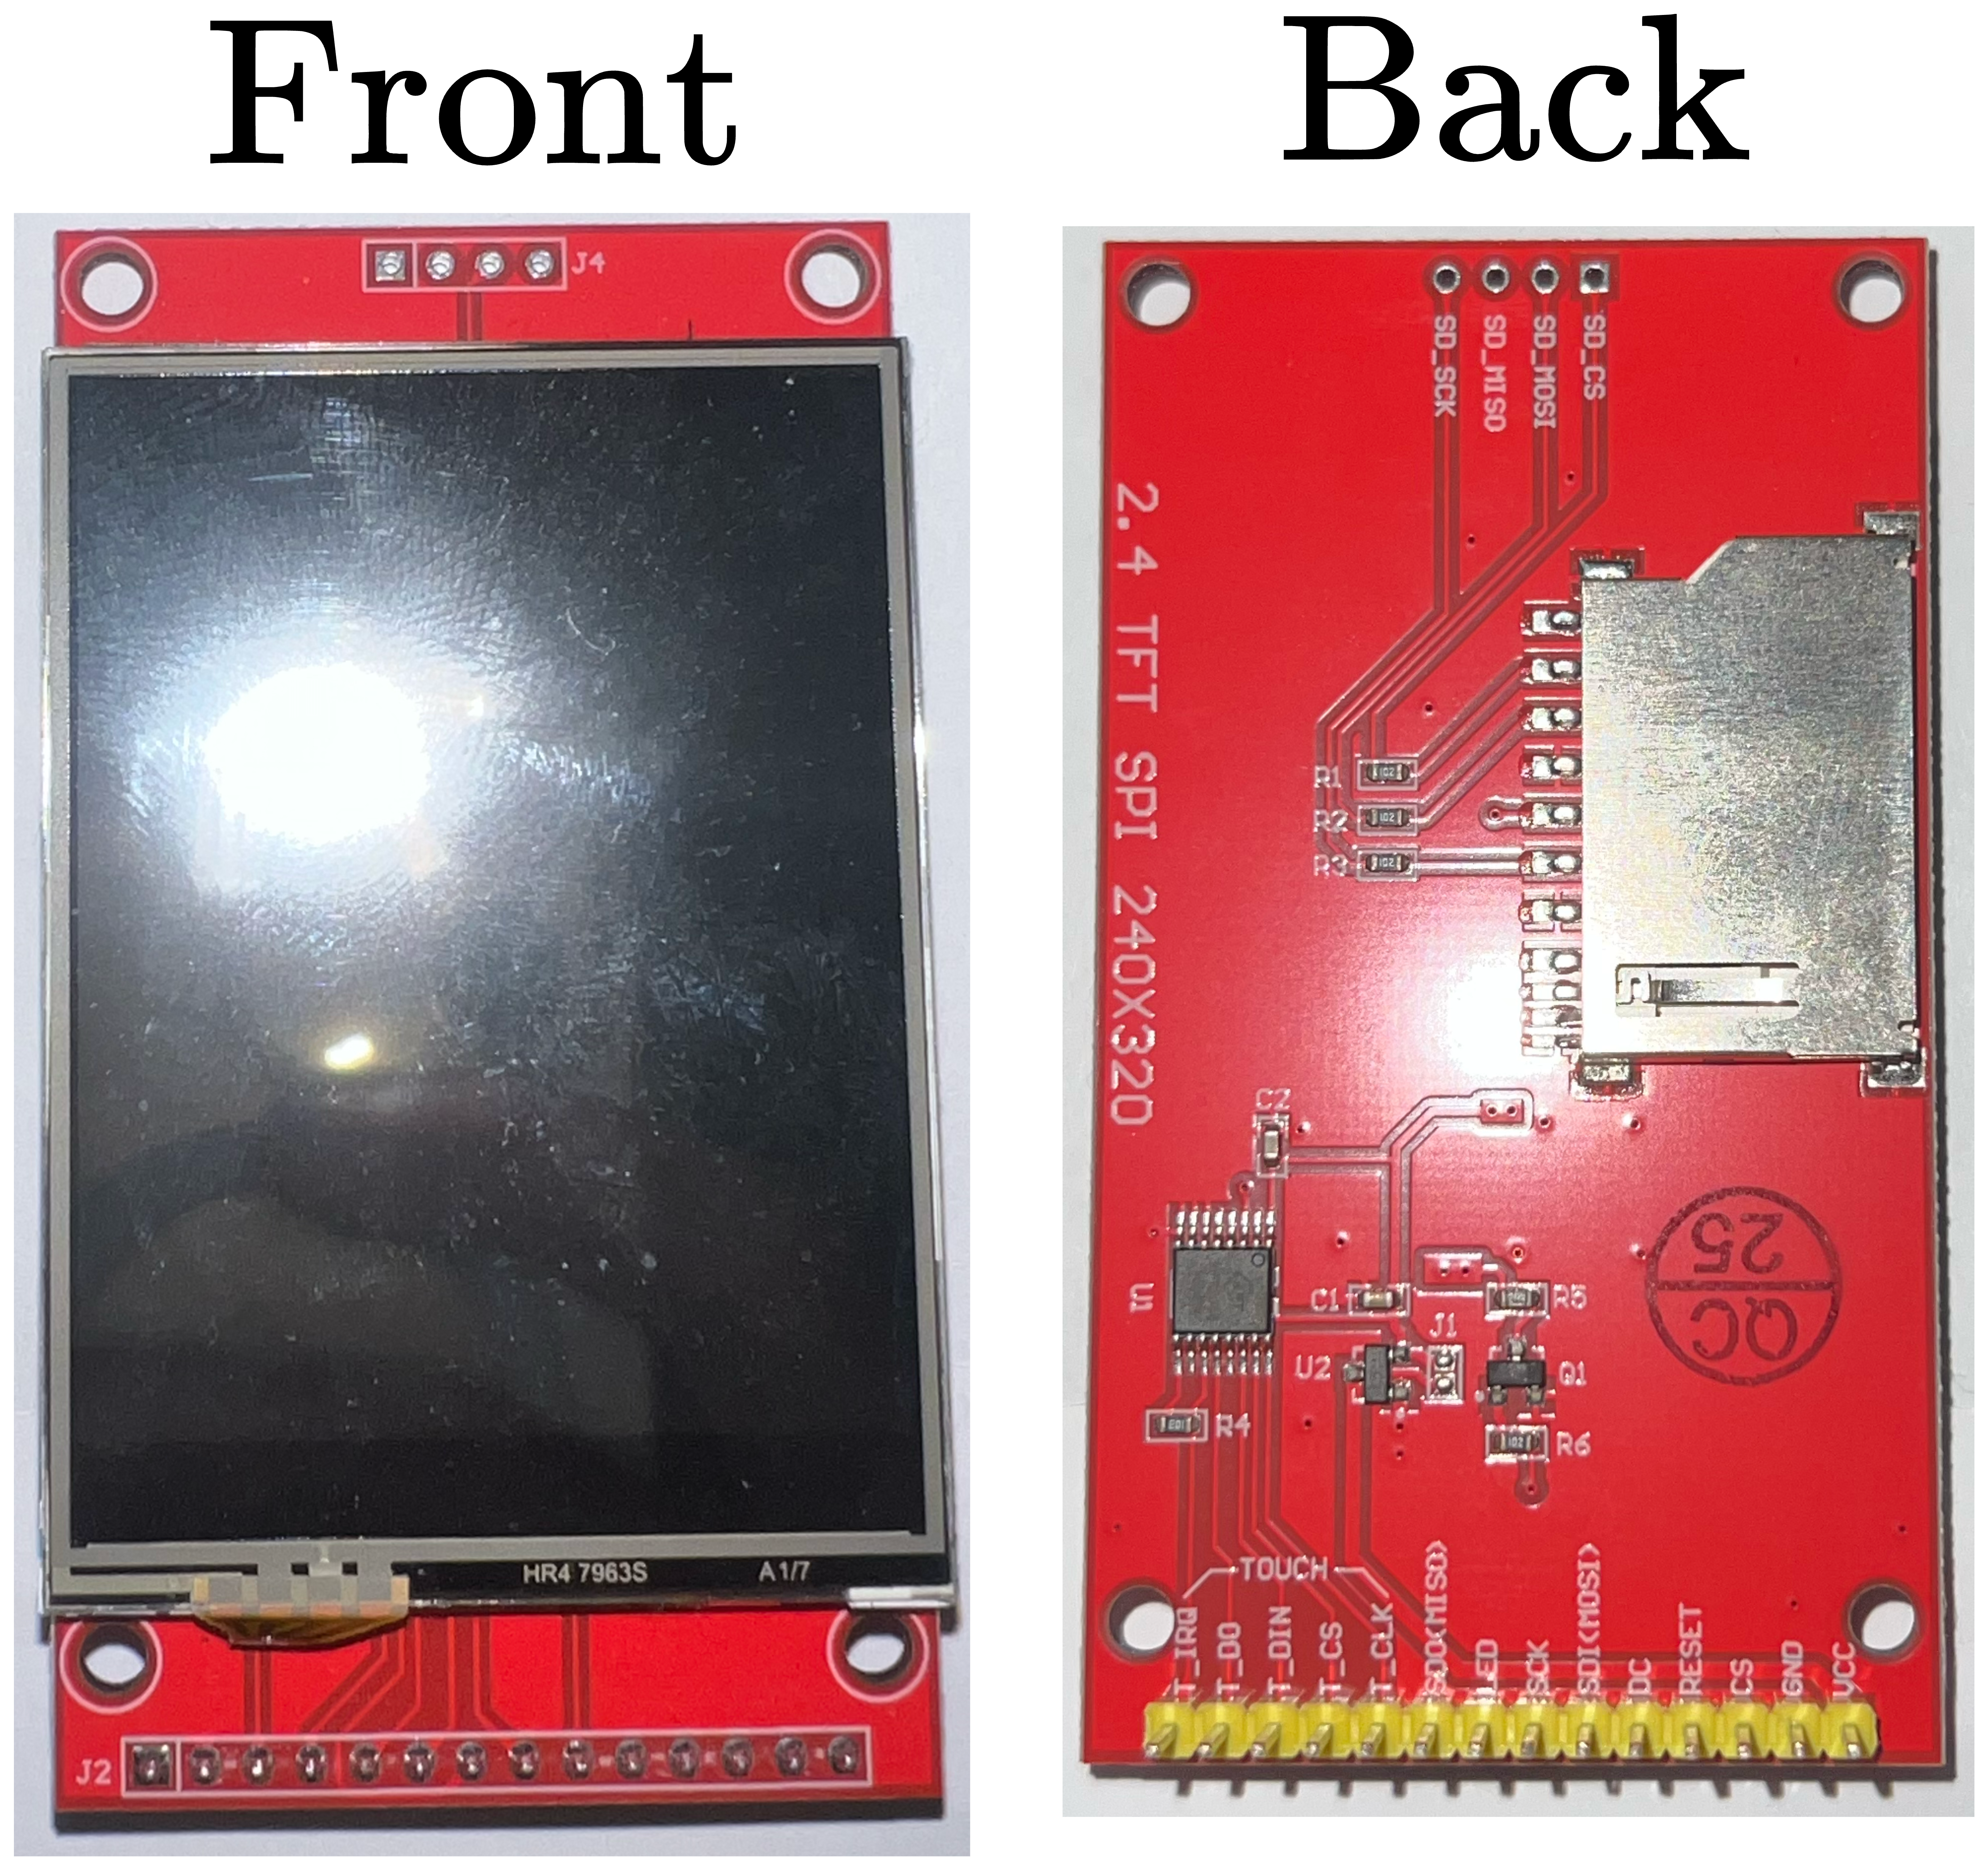
\includegraphics[width=0.5\linewidth]{img/touch-screen-picture.png}
    \caption{Pictures of the used TFT touch screen display}
    \label{fig:tft-picture}
\end{figure}

\begin{table}[ht!]
\centering
\caption{Pin assignments for display and touch controllers}
\begin{tabular}{|l|l|l|l|}
\hline
\textbf{Component} & \textbf{Function} & \textbf{Arduino Pin} & \textbf{Code Definition} \\
\hline
\multicolumn{4}{|c|}{\textbf{ILI9341 Display}} \\
\hline
\verb|VCC| & Power (3.3V) & \verb|3.3V| & — \\
\verb|GND| & Ground & \verb|GND| & — \\
\verb|LED| & LED Power (3.3V) & \verb|3.3V| & — \\
\verb|CS| & Chip Select & \verb|10| & \verb|TKB_TFT_CS| \\
\verb|D/C| & Data/Command & \verb|9| & \verb|TKB_TFT_DC| \\
\verb|RST| & Reset & \verb|8| & \verb|TKB_TFT_RST| \\
\verb|SDI(MOSI)| & SPI Data Out & \verb|11| & (Default SPI pin) \\
\verb|SDO(MISO)| & SPI Data In & \verb|12| & (Default SPI pin) \\
\verb|SCK| & SPI Clock & \verb|13| & (Default SPI pin) \\
\hline
\multicolumn{4}{|c|}{\textbf{XPT2046 Touch Controller}} \\
\hline
\verb|VCC| & Power (3.3V) & \verb|3.3V| & — \\
\verb|GND| & Ground & \verb|GND| & — \\
\verb|T_CS| & Chip Select & \verb|7| & \verb|TKB_TS_CS| \\
\verb|T_DIN| & SPI Data Out & \verb|11| & (Default SPI pin) \\
\verb|T_DO| & SPI Data In & \verb|12| & (Default SPI pin) \\
\verb|T_CLK| & SPI Clock & \verb|13| & (Default SPI pin) \\
\hline
\end{tabular}
\label{table:touchscreen-pins}
\end{table}

\subsubsection{Libraries}
The touch screen implementation uses the following Arduino libraries (see \verb|touch_keyboard.cpp|):
\begin{enumerate}
    \item \textbf{Adafruit GFX Graphic Library} \cite{adafruit_gfx_library}: Graphics library providing text, shapes, and drawing primitives.
    \item \textbf{Adafruit ILI9341 Library} \cite{adafruit_ili9341}: Display driver for the ILI9341 TFT controller.
    \item \textbf{XPT2046 Touchscreen Arduino Library} \cite{xpt2046_touchscreen}: Touch input driver for the XPT2046 controller.
    \item \textbf{FlashStorage Library} \cite{flashstorage}: Library for storing the calibration data on the non-volatile flash memory of the arduino.
    \item \textbf{SPI Library} \cite{arduino_spi_reference}: Standard Arduino SPI communication library.
\end{enumerate}

\subsubsection{Touch Screen Calibration}
Even though the resistive touch screen sits on top of the display, there is no shared circuitry between them, hence why we need to calibrate the touch screen to accurately map the touch coordinates coming from the touch screen to coordinates on the display. A resistive touch screen is comprised of two layers separated by a small gap, when a stylus is used to press somewhere on the screen, the two layers touch at that point, then by measuring two voltages $V_x$ and $V_y$, we get something similar to x-y coordinates (ADC readings).

During calibration, the XPT2046 touch controller provides 12-bit raw ADC readings (0--4095) at two reference points. The user is prompted to touch two crosshairs: one at the top-left corner (pixel 20,20) with ADC values $(x_1, y_1)$, and one at the bottom-right corner (pixel 210,300) with ADC values $(x_2, y_2)$. These ADC values are linearly mapped to accurate screen coordinates via affine transformations: 
$$\text{screen}_x = \frac{\text{rawADC}_x - c_x}{m_x}$$
$$\text{screen}_y = \frac{\text{rawADC}_y - c_y}{m_y}$$

The scaling factors are computed as:
$$m_x = (210 - 20) / (x_2 - x_1)$$
$$c_x = 20 - x_1 \cdot m_x$$
$$m_y = (300 - 20) / (y_2 - y_1)$$
$$c_y = 20 - y_1 \cdot m_y$$ 
These coefficients are stored in Arduino flash memory and applied to all subsequent touch inputs to convert raw ADC values to screen pixel coordinates. The screen calibration must only be done once since its results are stored on the flash memory to be reused on the next boot.


\subsubsection{User Interface Screens}

As seen in figure \ref{fig:screens-real}, the touch screen displays different screens during each phase to prompt the user. In the first phase, the user is prompted to initially approve the login by showing the server domain to make sure that the user will connect to the wanted server and not some other malicious domain (Screen (a)), if the user clicks on "ACCEPT", they are prompted to enter their username and password using the on-screen keyboard (Screens (b) and (c)) and then screen (d) is shown to confirm the receipt of the credentials. During phase 2, if the user makes a sensitive request that needs signing, screen (e) appears where the description of the sensitive request is shown and the user can choose to accept it or reject it. During phase 3, the user is prompted with screen (f) to accept or reject the session renewal. All screens are rendered using the Adafruit GFX Graphic Library to draw text, shapes, and buttons. As explained before, user interaction occurs through the resistive touch screen, where touches are read via SPI communication and then converted from 12 bit ADC values to accurate pixel coordinates using the stored affine transformations. The touch coordinates are then compared against the bounding boxes to determine which button was selected and execute the necessary action.

\begin{figure}
    \centering
    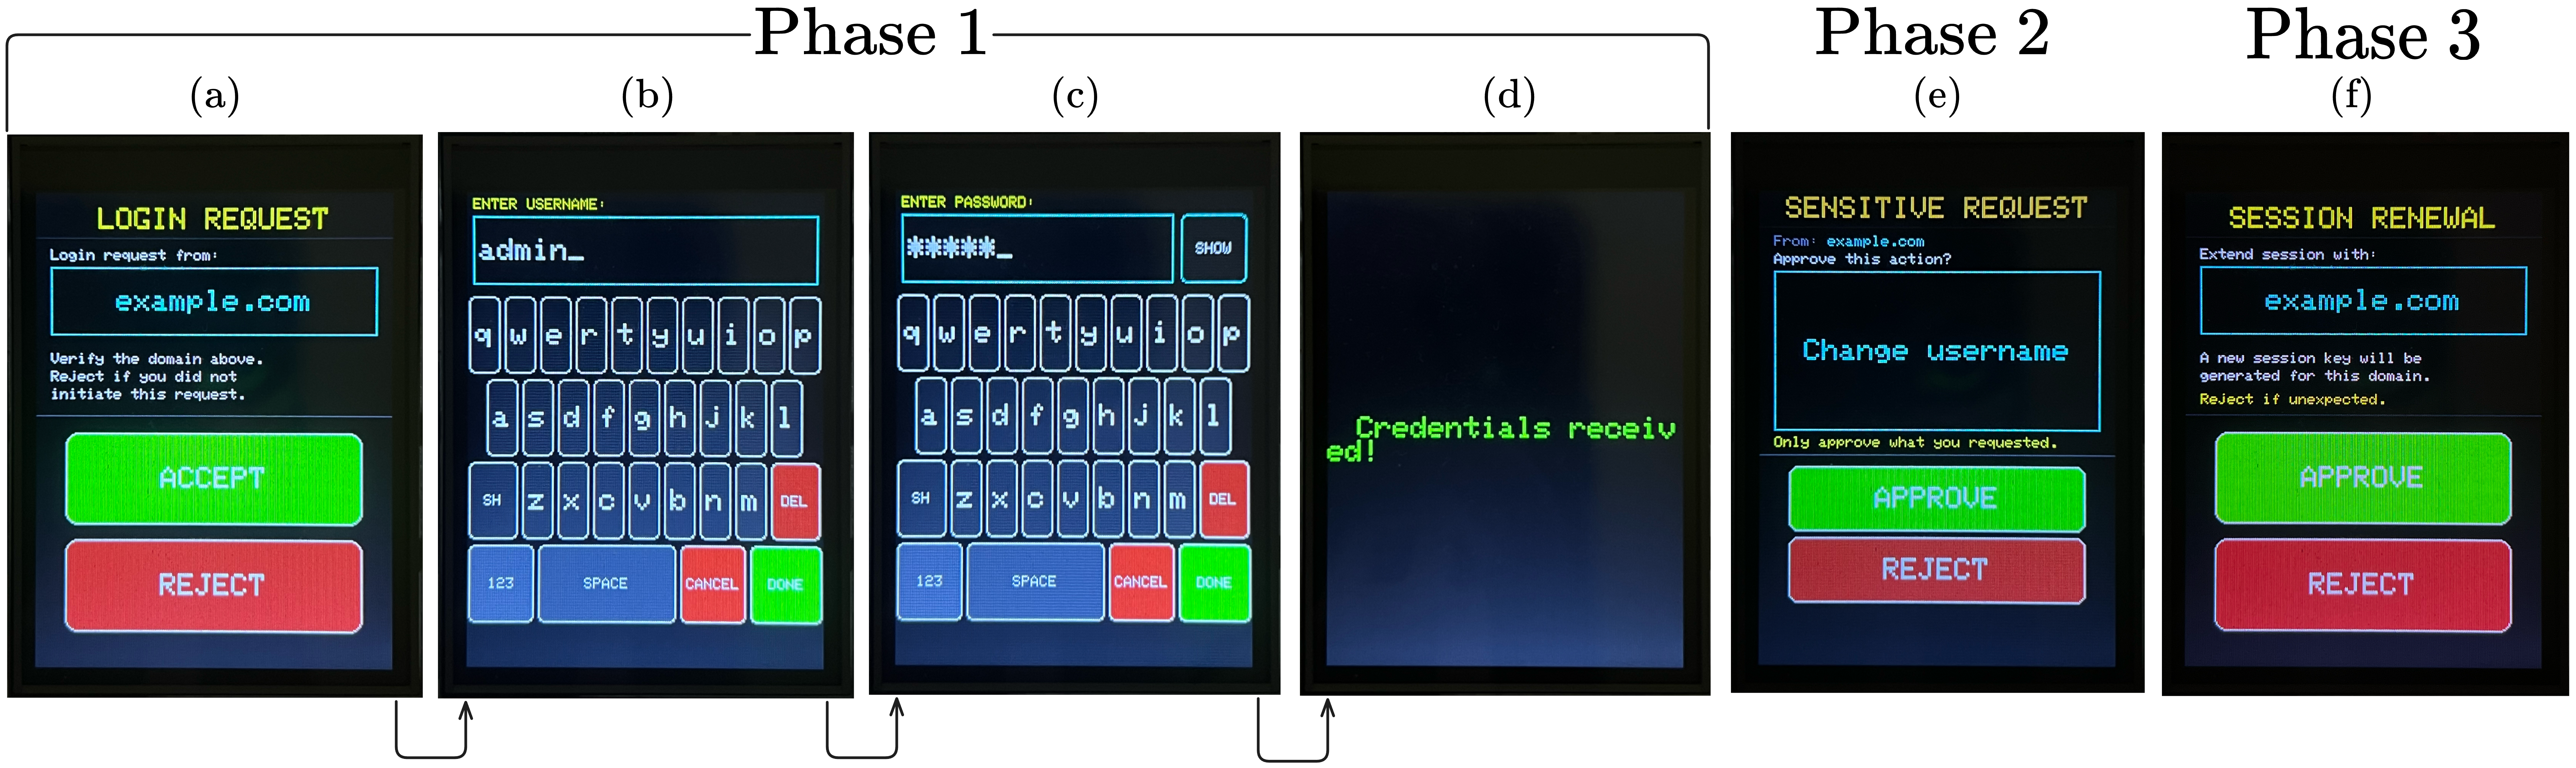
\includegraphics[width=1.1\linewidth]{img/screens-real.png}
    \caption{Pictures of all the possible screens}
    \label{fig:screens-real}
\end{figure}
  
\section{DOMAN Implementation}
DOMAN (Dongle Manager) is implemented as a local FastAPI \cite{fastapi_docs} server that exposes a WebSocket \cite{rfc6455} endpoint at \texttt{ws://127.0.0.1:8765/ws} to the browser. It simply translates JSON commands from the browser into newline-terminated ASCII commands and sends them to the Arduino over the USB CDC serial port. For example, a signature request arrives from the browser to DOMAN over the WebSocket as:
\begin{verbatim}
{
  "cmd":         "sign_payload",
  "domain":      "...",
  "payload_b64": "..."
}
\end{verbatim}
and is forwarded to the Arduino as the newline-terminated ASCII string:
\begin{verbatim}
sign_payload <domain> <payload>\n
\end{verbatim}

DOMAN uses an asynchronous event loop (\verb|asyncio|) for all WebSocket and HTTP handling, while serial communication runs in a dedicated thread since the blocking serial IO would otherwise block the event loop. 

Since the dongle can only process one request at a time, concurrent requests are serialised using a lock so that only one command is sent to the dongle at a time.

WebSocket was chosen over a conventional HTTP endpoint because dongle operations are long-running and produce incremental output. An HTTP response would have to buffer the entire operation before returning, leaving the browser with no feedback during the wait, or the browser could continuously poll DOMAN, both approaches are not ideal. A WebSocket connection however allows DOMAN to forward each output line from the dongle to the browser as it arrives, giving the user real-time progress of each phase.

DOMAN also exposes two HTTP debug endpoints for testing purposes: \texttt{GET /debug/list-states} to list all LR-PUF state slots on the FPGA and \texttt{POST /debug/clear-states} to erase them. A Swagger UI at \verb|http://127.0.0.1:8765/docs| can be used to easily call these endpoints (Figure \ref{fig:swaggerUI}).

\begin{figure}
    \centering
    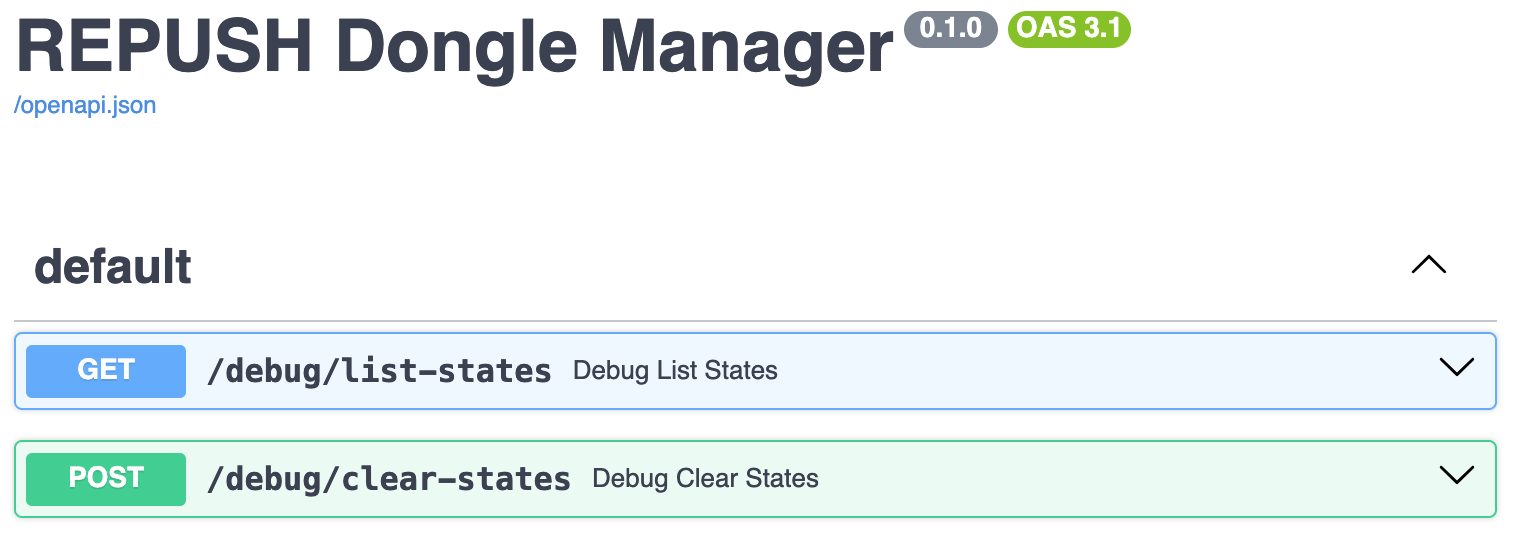
\includegraphics[width=1\linewidth]{img/swaggerUI-DOMAN.png}
    \caption{DOMAN Swagger UI}
    \label{fig:swaggerUI}
\end{figure}
As mentioned in the design section, DOMAN does not perform any cryptographic operations. It simply acts as a translation and orchestration layer between the browser and the dongle. The DOMAN implementation can be found in the repository named \verb|REPUSH-DOMAN|.

\section{Browser / Frontend Implementation}

The browser frontend is an HTML page served statically by the REPUSH server which contains all the necessary JavaScript to allow the browser to communicate and coordinate with DOMAN via the previously mentioned WebSocket endpoint. For this implementation, the page is intended as a demonstration of the protocol, as such, it is very explicit and transparent about the three phases and their inner workings, as seen in figure \ref{fig:landing-page}. A production website would perform most of these steps silently in the background. For styling the page, Tailwind CSS \cite{tailwindcss} was used.
\begin{figure}
    \centering
    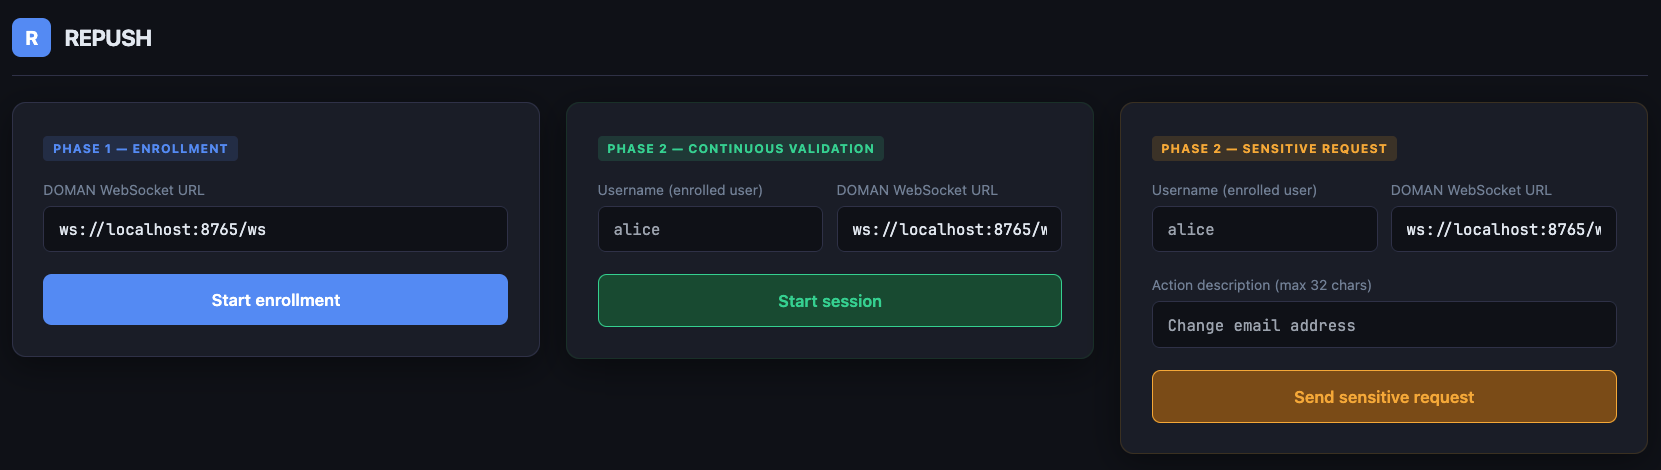
\includegraphics[width=1\linewidth]{img/landing-page.png}
    \caption{REPUSH demonstration page}
    \label{fig:landing-page}
\end{figure}

The page is divided into three side-by-side panels:
\paragraph{Phase 1 panel:} It accepts the DOMAN WebSocket URL as input and triggers the enrollment on the dongle when the user clicks on "Start enrollment". The JavaScript calls the REPUSH server with \texttt{POST /api/enroll/init} to obtain the certificate and enrollment payload from the server, then forwards them to the dongle via DOMAN. The user then has to approve the login request on the touch screen for the server's domain and enter their credentials on the dongle. The dongle's output is then sent back to the server on \texttt{POST /api/enroll/verify} so that the server can verify the credentials and continue accordingly by returning the acknowledgment. This acknowledgment is then returned to the dongle via DOMAN. If the acknowledgment on the dongle is successful, the enrollment is finalized by calling \texttt{POST /api/enroll/confirm}, after which the frontend immediately requests a phase 2 session token via \texttt{POST /api/session/start} and holds it in memory as a JavaScript variable. No cookies are set for this demonstration, rather session continuity is maintained purely through this variable. The final state of the panel after a successful enrollment can be seen in figure \ref{fig:phase-1-panel}. In "EVENT LOG", each output line from the dongle is appended to the log panel in real time with a timestamp as it arrives over the WebSocket connection. Each dongle command follows a self-contained lifecycle: the frontend opens a WebSocket connection to DOMAN, sends the JSON command, and appends each incoming line to the log panel until DOMAN sends a terminal message indicating the command has completed, at which point the connection is closed. The log also contains events from the server.

\begin{figure}
    \centering
    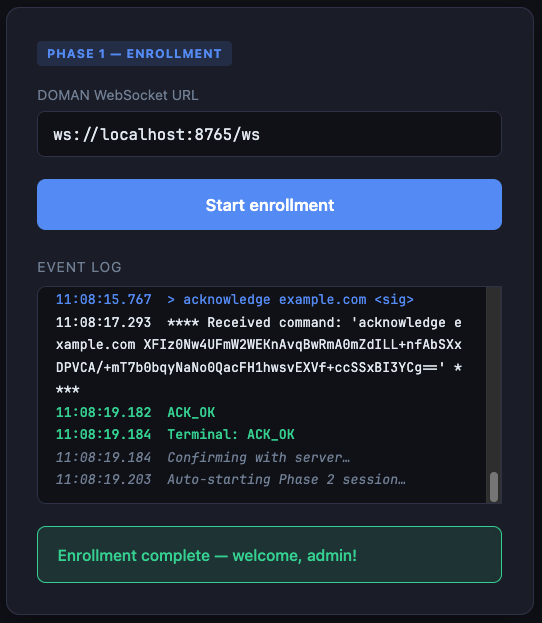
\includegraphics[width=0.5\linewidth]{img/phase-1-panel.png}
    \caption{Phase 1 panel after successful enrollment}
    \label{fig:phase-1-panel}
\end{figure}

\paragraph{Phase 2 and 3 panel:} This panel shows two live progress bars updated every 500 ms by polling \texttt{GET /api/session/status}. As seen in figure \ref{fig:phase-2-panel}, the first bar shows the elapsed time since the last revalidation relative to $T_\text{Validity}$, when this bar is full, on the subsequent request, the dongle will be asked to sign a non-sensitive payload for proof of ownership. The second bar below shows the age of the session relative to $T_\text{Expiry}$, when this bar is full, on the subsequent request, the dongle will prompt the user to extend the session and new keys will be generated for the new session. The "Make request" button simulates a non-sensitive request by calling \texttt{POST /api/session/ping}. The server may respond with \texttt{ok}, \texttt{revalidation\_required}, or \texttt{reconfiguration\_required}. If revalidation is required, the browser forwards the non-sensitive payload to the dongle via DOMAN and submits the resulting signature to the server by calling \texttt{POST /api/session/submit\_signature}. If reconfiguration is needed, the browser sends the reconfiguration payload to the dongle and submits the resulting token by calling \texttt{POST /api/session/verify\_reconf}, delivers the acknowledgment back to the dongle and finalizes the session renewal by calling \texttt{POST /api/session/confirm\_reconf} which replaces the session token with a new one. Since the session only expires every 300 seconds, the button "Force reconfig now" can be used to make it expire sooner for demonstration purposes. The "EVENT LOG" contains timestamped logs from both the server and the dongle. 

\begin{figure}
    \centering
    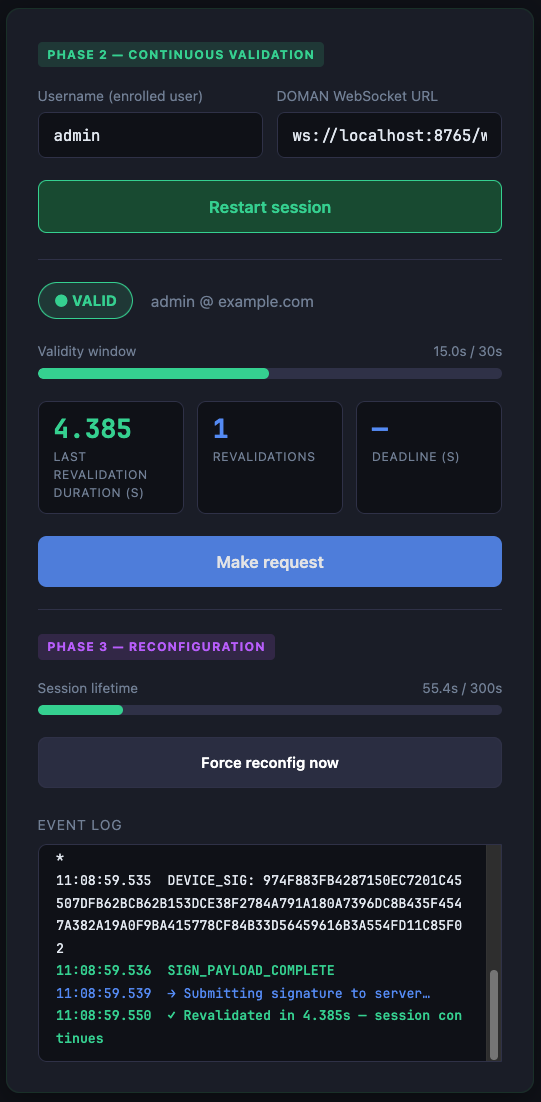
\includegraphics[width=0.5\linewidth]{img/phase-2-panel.png}
    \caption{Phases 2 and 3 panel after the session starts}
    \label{fig:phase-2-panel}
\end{figure}

\paragraph{Sensitive request panel:} The third panel (Figure \ref{fig:phase-2-sensitive-panel}) allows for testing a sensitive signing request. The username is auto-filled after enrollment and the tester can specify which message to show on the dongle. In a real use-case, this would be handled by the server, not by the  user in the frontend. The frontend calls \texttt{POST /api/sensitive/request} to obtain a sensitive payload from the server, then the dongle prompts the user with the sensitive action and its description and submits the resulting signature accordingly to \texttt{POST /api/sensitive/verify}. The "EVENT LOG" shows the real-time progress from the dongle and server.

\begin{figure}
    \centering
    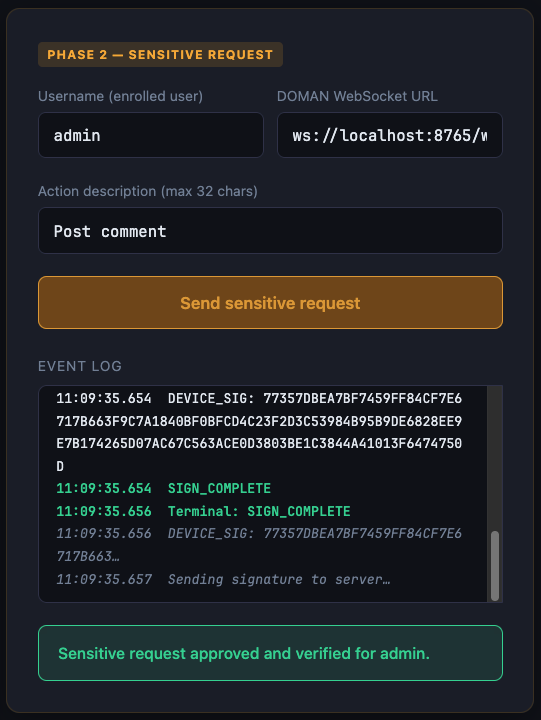
\includegraphics[width=0.5\linewidth]{img/phase-2-sensitive-panel.png}
    \caption{Phase 2 sensitive request panel after a successful signature request}
    \label{fig:phase-2-sensitive-panel}
\end{figure}

\section{Server / Backend Implementation}

The REPUSH server is a FastAPI \cite{fastapi_docs} server written in Python. For demonstration purposes, it runs locally, but in a real setting, it would be a remote server.

\subsection{Libraries}
The server implementation relies on the following Python libraries:

\begin{enumerate}
  \item \textbf{FastAPI} \cite{fastapi_docs}: Server framework used to define all API endpoints and handle request validation.
  \item \textbf{SQLAlchemy} \cite{sqlalchemy}: ORM (Object-Relational Mapping) used to manage the SQLite enrollment database and abstract all database operations.
  \item \textbf{pyca/cryptography} \cite{pycryptography}: Provides the server-side implementations of Ed25519 signing and verification, X25519 Diffie-Hellman, and ChaCha20-Poly1305 authenticated encryption used in the ECIES construction.
  \item \textbf{pyca/bcrypt} \cite{bcrypt}: Used to hash and verify user passwords stored in the database.
  \item \textbf{Pydantic} \cite{pydantic}: Handles request and response schema validation for all API endpoints.
\end{enumerate}



\subsection{State and Storage}
The server stores durable enrollment records such as the username, password hash, enrolled dongle public key $PK_i$, domain and the session challenge $C^i_\text{Session}$ in a SQLite \cite{sqlite} database under a table called \texttt{users} (Table \ref{tab:db-schema-users}). When phase 2 starts, $PK_i$ and $C^i_\text{Session}$ are copied from the database into a global dict which uses session tokens as its keys. This dict also contains all the necessary timestamp variables to determine if a revalidation or reconfiguration is due. The three global time parameters that control the frequency of validations and reconfigurations are defined as: 
\begin{itemize}
  \item $T_{\text{Validity}}$ (default 30 seconds): maximum interval between dongle revalidations.
  \item $T_{\text{Timeout}}$ (default 60 seconds): grace window for the dongle to respond before the session is terminated.
  \item $T_{\text{Expiry}}$ (default 300 seconds): maximum session lifetime before a full Phase~3 reconfiguration is required.
\end{itemize}


\begin{table}[ht!]
\centering
\caption{\texttt{users} SQL table schema.}
\begin{tabular}{ll}
\hline
\textbf{Field} & \textbf{Description} \\
\hline
\texttt{username}      & Primary identifier \\
\texttt{password\_hash} & Bcrypt-hashed password \\
\texttt{device\_pubkey} & Enrolled Ed25519 public key $PK_i$ (hex) \\
\texttt{domain}        & Enrolled domain string \\
\texttt{challenge\_hex} & Raw session challenge $C^i_{\text{Session}}$ (hex) \\
\texttt{enrolled\_at}  & Timestamp of the most recent enrollment or reconfiguration \\
\texttt{created\_at}   & Timestamp of account creation \\
\hline
\end{tabular}
\label{tab:db-schema-users}
\end{table}

\subsection{Phase 1: Enrollment and Login}
The following endpoints are used to implement the enrollment phase:
\begin{itemize}
    \item \texttt{POST /api/enroll/init}: generates a fresh certificate and signed login payload, storing the session challenge in memory.
    \item \texttt{POST /api/enroll/verify}: receives and decrypts the login token using the ECIES construction, cross-checks the dongle public key, verifies the device signature, authenticates the username and password against the database, and returns the acknowledgment signature.
    \item \texttt{POST /api/enroll/confirm}: finalizes enrollment by writing the dongle public key and session challenge to the database. 
\end{itemize}
\subsection{Phase 2: Operation}
The following endpoints are used to implement the second phase:
\begin{itemize}
    \item \texttt{POST /api/session/ping}: used to simulate a non-sensitive request. It checks $T_{\text{Expiry}}$ first: if the session has exceeded its lifetime, it returns \texttt{reconfiguration\_required} with a reconfiguration payload. Otherwise, if $T_{\text{Validity}}$ has elapsed since the last revalidation, it returns \texttt{revalidation\_required} with a signed non-sensitive payload and starts a termination countdown. If neither threshold is reached, it returns \texttt{ok}. When a revalidation is needed, a background task is scheduled to terminate the session after $T_{\text{Timeout}}$ seconds.
    \item \texttt{POST /api/session/submit\_signature}: verifies the dongle's Ed25519 signature and, on success, cancels the termination task and resets the last-validation timestamp.
    \item \texttt{POST /api/sensitive/request}: builds and signs a sensitive payload carrying the action description.
    \item \texttt{POST /api/sensitive/verify}: verifies the dongle's signature on the sensitive payload before authorizing the action.
\end{itemize}
\subsection{Phase 3: Reconfiguration}
\begin{itemize}
    \item \texttt{POST /api/session/verify\_reconf}: decrypts the reconfiguration token, verifies the device's signature over $PK_{i+1}$ using the old $PK_i$, and issues the reconfiguration acknowledgment.
    \item \texttt{POST /api/session/confirm\_reconf}: writes the new device public key and session challenge to the database, issues a new session token, and retires the old one. 
    \item \texttt{POST /api/session/force\_reconfig}:  resets the session start time so that the next ping immediately triggers $T_\text{Expiry}$, allowing the reconfiguration to be tested on demand without waiting for $T_\text{Expiry}$ to elapse.
\end{itemize} 

\subsection{CA Implementation}
In this implementation, the server also acts as the Certificate Authority. The CA private key is loaded from a local key file at startup alongside the server's own key pair. When \texttt{POST /api/enroll/init} is called, the server constructs a 128-byte certificate by concatenating the zero-padded domain string and its own Ed25519 public key, then signing the result with the CA private key. In a real use-case, the CA would be a separate offline entity rather than the server itself.





